\documentclass{beamer}


\usepackage[french,english]{babel}

\usepackage[T1]{fontenc}

\usepackage[utf8]{inputenc}
\usepackage[linesnumbered,ruled,vlined]{algorithm2e}
\SetKwComment{Comment}{$\triangleright$\ }{}
\usetheme{Warsaw}
\definecolor{rouge}{HTML}{DD0000}
\definecolor{vert}{HTML}{008000}

\addtobeamertemplate{footline}{\insertframenumber/\inserttotalframenumber}

\title{Création d'une \emph{Learning Heuristic} pour CVRP}

\author{Clément Legrand}





\titlegraphic{
	
\includegraphics[scale=0.5]{ensRennes.jpeg}
	
\includegraphics[scale=0.2]{logo_cristal.png}}

\begin{document}


\begin{frame}[plain]
\titlepage
Equipe ORKAD \footnote{Stage réalisé dans l'équipe ORKAD du centre CRIStAL à Lille, sous la direction de Laetitia Jourdan ( laetitia.jourdan@univ-lille.fr), Marie-Éléonore Kessaci (me.kessaci@univ-lille.fr) et Diego Cattaruzza (diego.cattaruzza@ec-lille.fr)}
\end{frame}

\section{Présentation du problème}

\subsection{Capacitated Vehicle Routing Problem (CVRP)}
\footnotesize
\begin{frame}{Capacitated Vehicle Routing Problem}
\begin{block}{Instance}
\begin{itemize}
\item $n$ points (de coordonnées ($x_i$,$y_i$)), dont 1 dépôt et $n-1$ clients (de  demande $d_i$)
\item $k$ véhicules disponibles, de capacité $C$ 
\end{itemize}
\end{block}

\begin{exampleblock}{Objectif}
On note $x_{i,j}^v$ qui vaut 1 si $j$ est desservi après $i$ par le véhicule $v$ (et 0 sinon).

Déterminer $Sol$ (ensemble des tournées) tel que:

\centering
$ Sol = argmin_{Sol} \sum_{i = 0}^{n} \sum_{j = 0}^{n} \sum_{v = 1}^{k} distance(i,j) x_{i,j}^v = argmin_{Sol}cost(Sol)$


\begin{alertblock}{Contraintes}
\begin{itemize}
\item Chaque client doit être desservie par un unique véhicule;
\item Chaque tournée doit partir et s'arrêter au dépôt;
\item La somme des demandes sur une tournée ne peut excéder la capacité du véhicule.
\end{itemize}
\end{alertblock}


\end{exampleblock}
\end{frame}

\begin{frame}{Illustration}
Instance A-n37-k06 (donc 36 clients, et 6 véhicules disponibles de capacité 100):
 \begin{columns}[t]
  \begin{column}{5cm}
  	\centering
	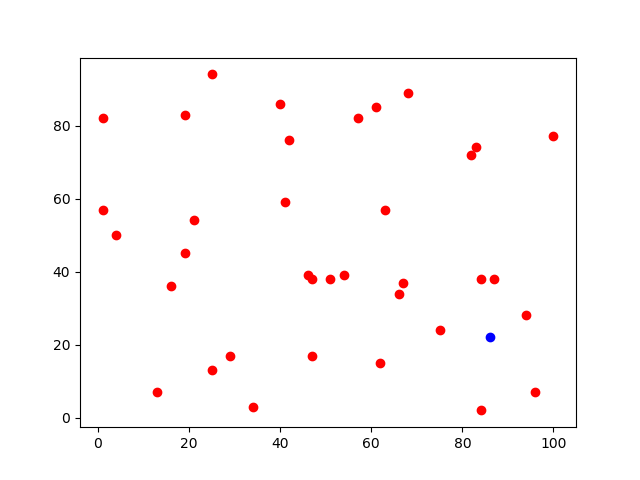
\includegraphics[scale=0.32]{instanceA3706.png}
	
	Représentation instance 
  \end{column}
  
  \begin{column}{5cm}
  	\centering
	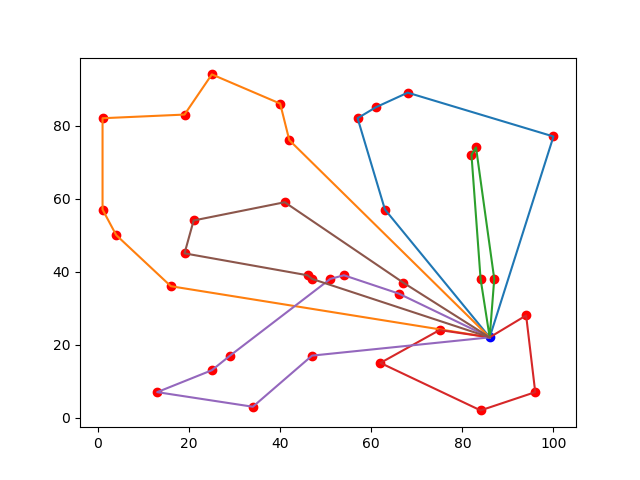
\includegraphics[scale=0.32]{bestA3706.png}
 
 	Meilleure solution connue,
 	
 	$cost = 950$
  \end{column}
 \end{columns}

\end{frame}

\subsection{Motivation}

\begin{frame}
\begin{block}{Objectif}
Intégrer de la connaissance pour trouver une meilleure solution
\end{block}

\begin{exampleblock}{Méthode}
Réussir à prédire des arêtes qui appartiendront à la solution optimale, et les exploiter pour construire une nouvelle solution.
\begin{itemize}
\item Comparer des solutions initiales à des solutions optimales pour des petites instances;
\item Établir des règles qui caractérisent ces arêtes;
\item Exploiter ces arêtes dans un algorithme d'optimisation.
\end{itemize}
\end{exampleblock}

\begin{alertblock}{Problèmes}
\begin{itemize}
\item Comment construire une solution initiale de bonne qualité ?
\item Quel algorithme d'optimisation utiliser ?
\item Comment extraire la connaissance ?
\item Comment intégrer la connaissance dans un algorithme d'optimisation ?
\end{itemize}
\end{alertblock}
\end{frame}

\section{Construction solution initiale}

\subsection{Algorithme CW}


\begin{frame}{Algorithme Clarke \& Wright (CW)}

CW\footnote{IK. Altinel and T. Öncan, A new enhancement of the Clarke and Wright savings heuristic for the capacitated vehicle routing problem (2005)}$\rightarrow$ Algorithme glouton (chaque client est initialement desservi par un véhicule (nombre de véhicules non respectée), puis la fusion des tournées est basée sur un calcul de saving). 



\begin{exampleblock}{Définition saving}
Calcul du saving de $i$ et $j$ avec:

\centering
$s(i,j) = c_{i0} + c_{0j} - \textcolor{rouge}{\lambda} c_{ij} + \textcolor{rouge}{\mu} \vert c_{i0} - c_{0j} \vert + \textcolor{rouge}{\nu} \frac{d_i + d_j}{\overline{d}}$

\textcolor{rouge}{$(\lambda,\mu,\nu)$ sont des paramètres à déterminer}
\end{exampleblock}

\begin{block}{Fonctionnement}
Tant que $max_{(i,j)}s(i,j) > 0$:
\begin{itemize}
\item $(i,j) \leftarrow argmax_{(i,j)}s(i,j)$;
\item Les tournées qui contiennent $i$ et $j$ sont fusionnées (si possible);
\item $s(i,j) \leftarrow  0$.
\end{itemize} 

\end{block}
\end{frame}

\subsection{Exemple d'exécution}
\begin{frame}{Exécution pour $(\lambda,\mu,\nu) = (1,1,1)$ sur A-n37-k06}

 \begin{columns}[t]
  \begin{column}{4cm}
  	\centering
  	Initialisation
  	
	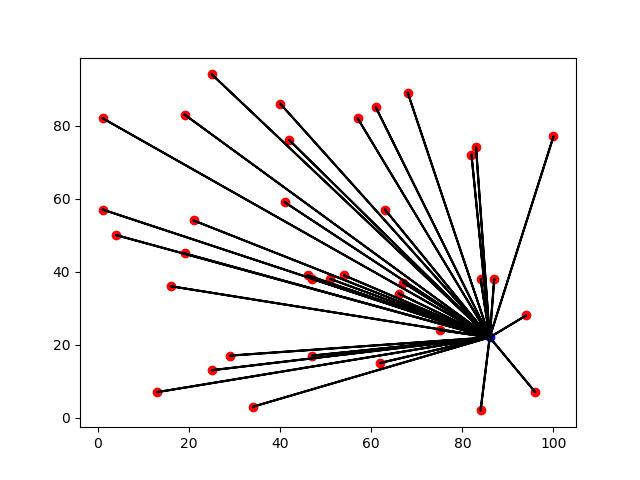
\includegraphics[scale=0.2]{CWinit.png}
	
	
  \end{column}
  
  \begin{column}{4cm}
  	\centering
  	1$^{ere}$ fusion
  	
	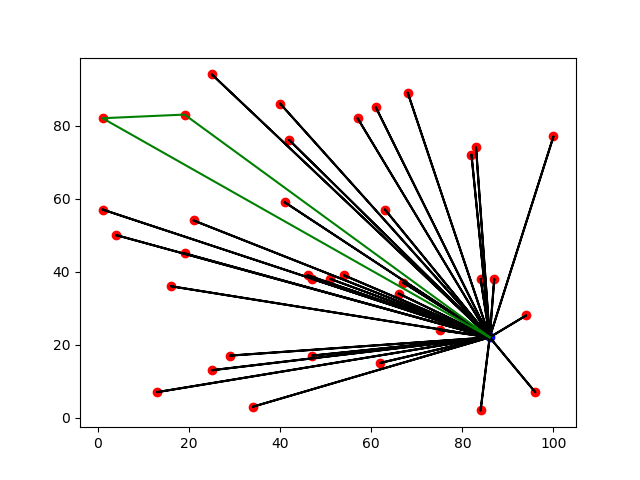
\includegraphics[scale=0.2]{CW1.png}
 
 	 \centering
 $\Downarrow$
 
 Solution (31 fusions, $cost = 1297$)
 
 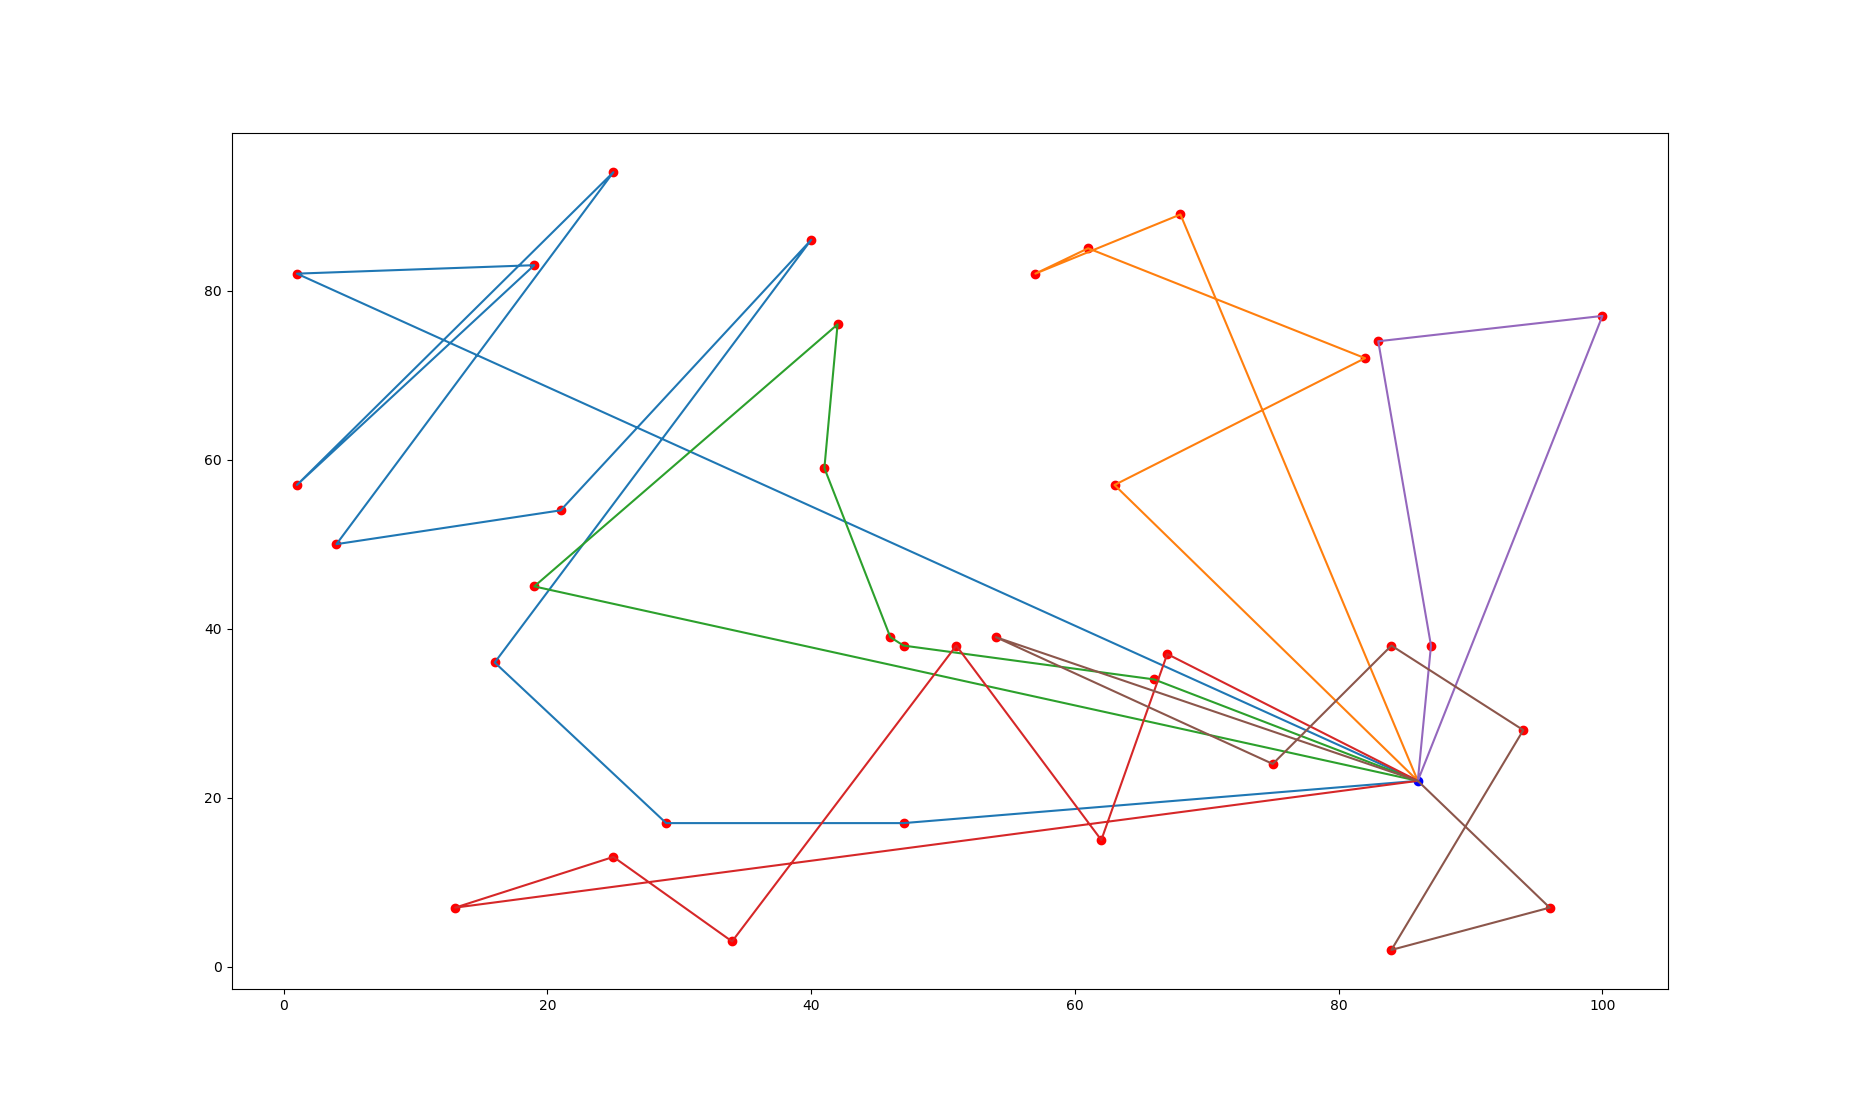
\includegraphics[scale=0.09]{resCW101010.png}
  \end{column}


  \begin{column}{4cm}
  	\centering
  	2$^{eme}$ fusion
  	
	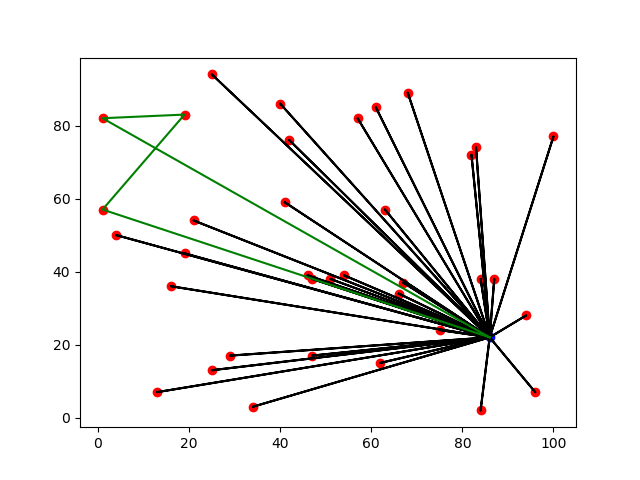
\includegraphics[scale=0.2]{CW2.png}
 	
	
	\begin{block}{Observation}
	Pour améliorer la solution obtenue, on pourrait réorganiser chaque tournée, pour diminuer leur coût.
	\end{block}
  \end{column}
 \end{columns}
 
 


\end{frame}

\subsection{Problème de $(\lambda,\mu,\nu)$}

\begin{frame}{Choix de $(\lambda,\mu,\nu)$ ?}
Dans la littérature plusieurs résultats sont disponibles :
\begin{itemize}
\item On peut se restreindre à l'intervalle $[0,2]$ pour choisir $\lambda (\neq 0)$, $\mu$ et$ \nu$.
\item Il est inutile de regarder ce qui se passe au centième.
\end{itemize}

\begin{exampleblock}{Bilan}
Ainsi on se contentera pour la suite de prendre des valeurs de $\lambda, \mu$ et$ \nu$ arrondies au dixième, et comprises entre $[0,2]$ (et $\lambda \neq 0$). Donc 8820 triplets possibles.
\end{exampleblock}

\end{frame}

\begin{frame}{Choix de $(\lambda,\mu,\nu)$ ?}
\begin{columns}[t]

  \begin{column}{4cm}
  	\centering
	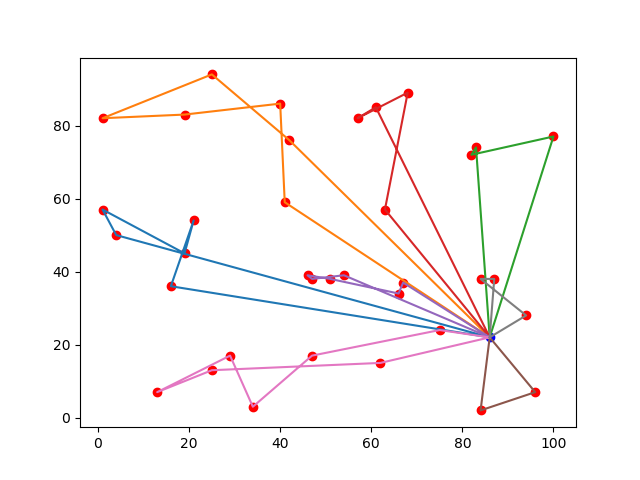
\includegraphics[scale=0.27]{resCW190105.png}
 
 	$(1.9,0.1,1.5), cost = 1106$
  \end{column}
  
 
  \begin{column}{4cm}
  	\centering
	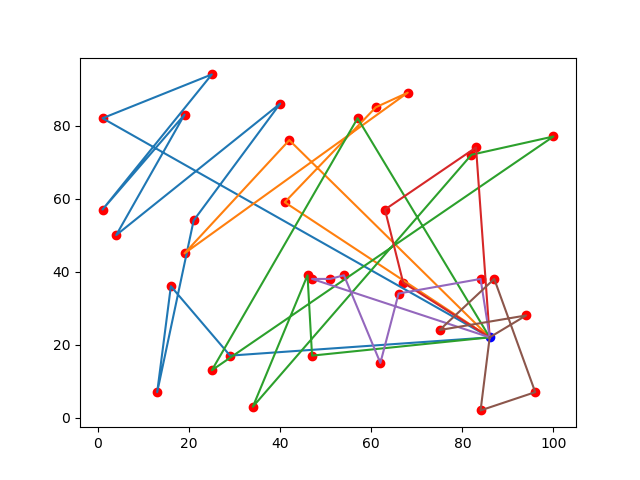
\includegraphics[scale=0.27]{resCW111.png}
	
	$(0.1,0.1,0.1), cost = 1569$
  \end{column}
  


 
  \begin{column}{4cm}
  	\centering
	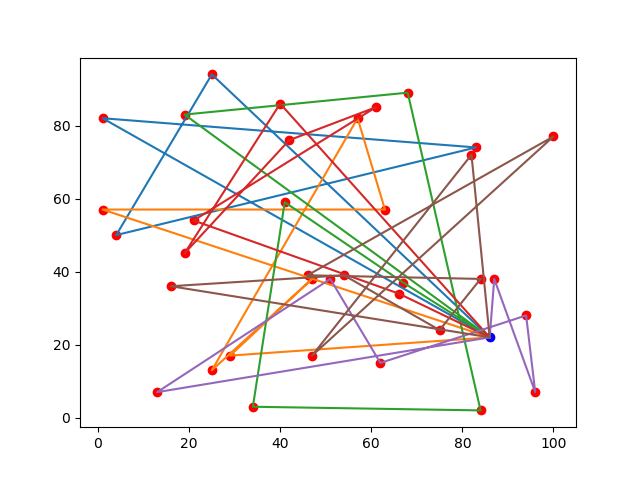
\includegraphics[scale=0.27]{resCW001015.png}
	
 	$(0.0,1.0,1.5), cost = 2191$

  \end{column}
 \end{columns}
 
\begin{alertblock}{Bilan}
Difficile de prévoir l'influence des paramètres $(\lambda,\mu,\nu)$ (pas d'évolution linéaire...). 

C'est aussi le cas pour toute instance : l'influence de $(\lambda,\mu,\nu)$ dépend de l'instance.
\end{alertblock}

\end{frame}

\section{Proposition de l'algorithme d'optimisation}

\subsection{Heuristique A \& S}

\begin{frame}{Heuristique Arnold \& Sörensen} 
Heuristique A \& S \footnote{Florian Arnold and Kenneth Sörensen, A simple, deterministic and efficient knowledge-driven heuristic for the vehicle routing problem (2017)}
\begin{algorithm}[H]
\DontPrintSemicolon % Some LaTeX compilers require you to use \dontprintsemicolon instead

$Sol \gets CW(\lambda,\mu,\nu)$\;
$NewSol \gets Sol$\;
\While {Pas d'amélioration depuis 3 min} {
	Calcul de la pire arête\;
	$NewSol \gets EjectionChain_{BI-O}$\;
	$NewSol \gets LinKernighan_{BI-O}$\;
	$NewSol \gets CrossExchange_{BI-O}$\;
	$NewSol \gets LinKernighan_{BI-O}$\;
	\If {$cost(NewSol) < cost(Sol)$} {
		$Sol \gets NewSol$\;
	}
}
\Return{$Sol$}\;

\end{algorithm}

\end{frame}

\subsection{Détail des opérations}

\begin{frame}{Pire arête}
\begin{exampleblock}{Pire arête}
La pire arête du graphe est l'arête $(i,j)$ qui maximise la fonction:
\begin{center}
$b(i,j) = \frac{[\gamma_w w(i,j) + \gamma_c c(i,j)] [\frac{d(i,j)}{max_{k,l}d(k,l)}] ^ {\frac{\gamma_d}{2}}}{1+p(i,j)}$
\end{center}
\end{exampleblock}

\begin{figure}
\centering
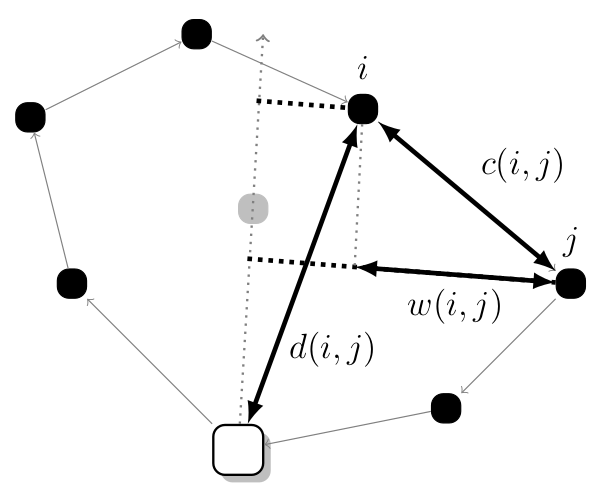
\includegraphics[scale=0.2]{metrics_big.png}
\end{figure}

\end{frame}

\begin{frame}{Opérateurs de voisinage}
\begin{block}{Ejection-chain}
Déplacer $l$ clients sur des tournées. On fixe \textcolor{vert}{ $l = 3$} d'après la littérature.
\end{block}
\begin{block}{Cross-exchange}
Échanger deux séquences de clients entre deux tournées. 
\end{block}
\begin{figure}
	\centering
	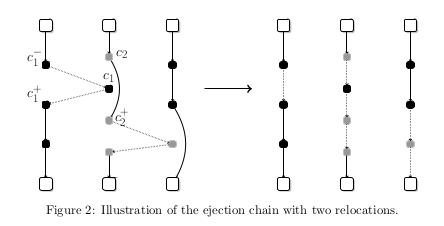
\includegraphics[scale=0.3]{ejection_chain.png}
	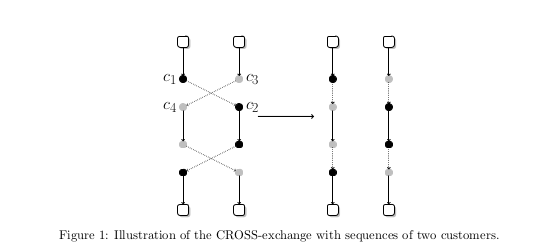
\includegraphics[scale=0.3]{cross_exchange.png}
\end{figure}

\end{frame}

\begin{frame}{Opérateurs de voisinage}
\begin{block}{Lin-Kernighan}
\begin{itemize}
\item Créé pour TSP;
\item Optimisation intra-tournée (chaque tournée est améliorée indépendamment des autres).
\end{itemize}
\end{block}
\begin{figure}
	\centering
	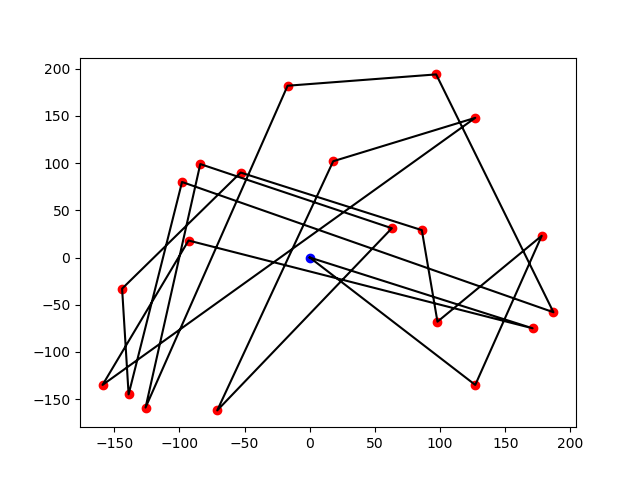
\includegraphics[scale=0.3]{test4_20_init.png}
	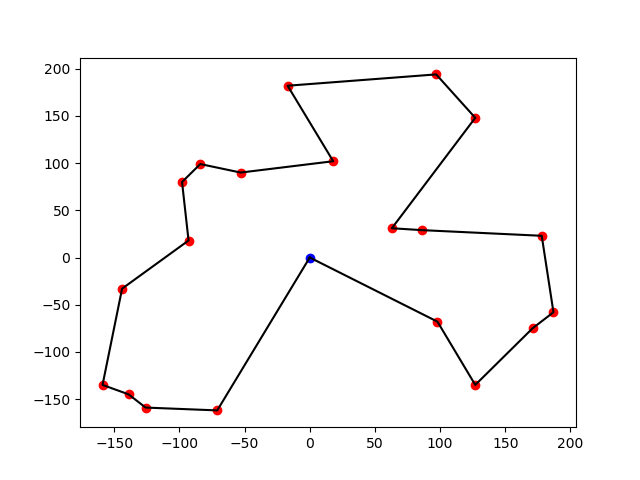
\includegraphics[scale=0.3]{test4_20_LKopt.png}
\end{figure} 
\end{frame}

\subsection{Algorithme d'optimisation utilisé}

\begin{frame}{Algorithme d'optimisation ($H_c$)}

\begin{algorithm}[H]
\DontPrintSemicolon % Some LaTeX compilers require you to use \dontprintsemicolon instead

$Sol \gets CW(\lambda,\mu,\nu)$\;
$NewSol \gets Sol$\;
\While {La dernière amélioration date de moins de \textcolor{rouge}{$n/3$ sec}} {
	Calcul de la pire arête\;
	$NewSol \gets EjectionChain_{\textcolor{rouge}{FI-RD}}$\;
	$NewSol \gets LinKernighan_{BI-O}$\;
	$NewSol \gets CrossExchange_{\textcolor{rouge}{FI-RD}}$\;
	$NewSol \gets LinKernighan_{BI-O}$\;
	\If {$cost(NewSol) < cost(Sol)$} {
		$Sol \gets NewSol$\;
	}
	\textcolor{rouge}{
	\If {Pas d'amélioration depuis $n/2$ itérations} {  
		$NewSol \gets Sol$ \Comment*[r]{Restart} 
	}
	}
}
\Return{$Sol$}\;

\end{algorithm}

\end{frame}

\begin{frame}{Validation du \emph{Restart}}

\begin{table}[H]
\begin{tabular}{|@{}c@{}|@{}c@{}|@{}c@{}|@{}c@{}|@{}c@{}|@{}c@{}|@{}c@{}|@{}c@{}|@{}c@{}|@{}c@{}|}
   \hline
    & \multicolumn{3}{c|}{A-n37-k06} & \multicolumn{3}{c|}{A-n65-k09} & \multicolumn{3}{c|}{P-n101-k04} \\
   \hline
   Restart & Best & Mean$_{10}$ & Time & Best & Mean$_{10}$ & Time & Best & Mean$_{10}$ & Time \\
   \hline
   Sans &  950 & 957 & 195 & 1197 & 1215 & 395 & 722 & 736 & 783  \\   
   \hline
   Avec & 950 & 969 & 200 & 1200 & 1230 & 350 & 698 & 706 & 1500  \\
   \hline
\end{tabular}
\end{table}

\begin{exampleblock}{Bilan}
Diversification plus intéressante pour des grandes instances
\end{exampleblock}



\end{frame}


\section{Extraction des connaissances}

\subsection{Contribution}

\begin{frame}{Comment extraire de la connaissance ?}
 \begin{columns}[t]
  \begin{column}{4cm}
  	\centering
  	$CW(1.9,0.1,1.5)+LK$ 
  	$cost = 1041$, 19 arêtes opt
  	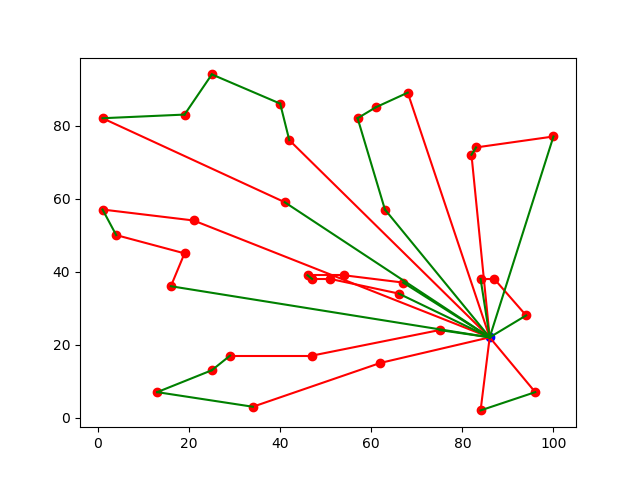
\includegraphics[scale=0.2]{edges190115.png}
	
	
  \end{column}
  
    \begin{column}{4cm}
  	\centering
  	$CW(0.1,0.1,0.1)+LK$ $cost = 1170$, 19 arêtes opt
	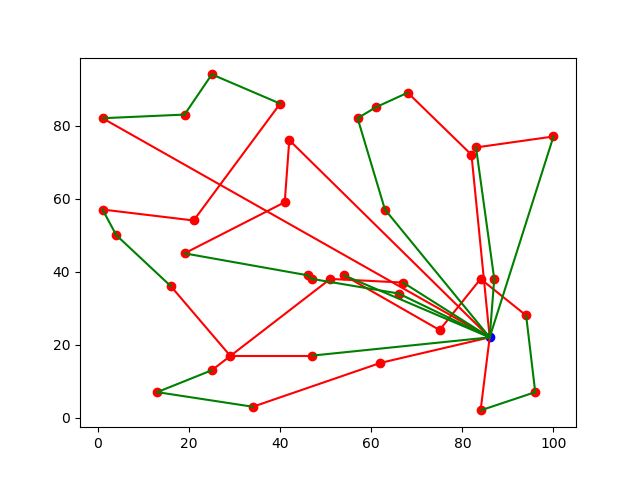
\includegraphics[scale=0.2]{edges101010.png}

	
	 $\downarrow$
 
 	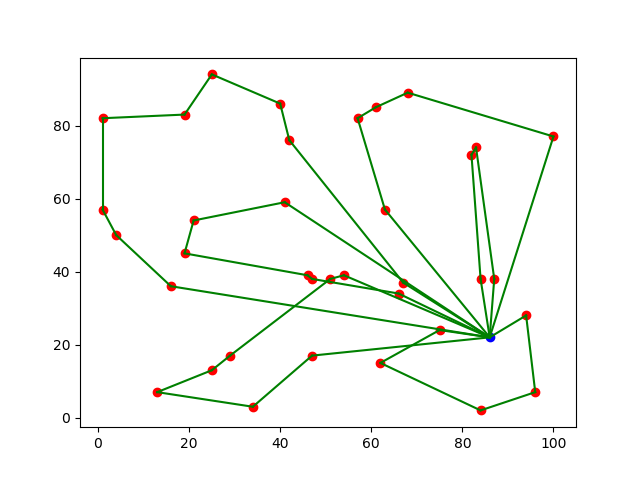
\includegraphics[scale=0.25]{edgesSol.png}
 
  	$cost = 950$, 42 arêtes 
  \end{column}
  
  \begin{column}{4cm}
  	\centering
  	$CW(0.0,1.0,1.5)+LK$ $cost = 1600$, 11 arêtes opt
	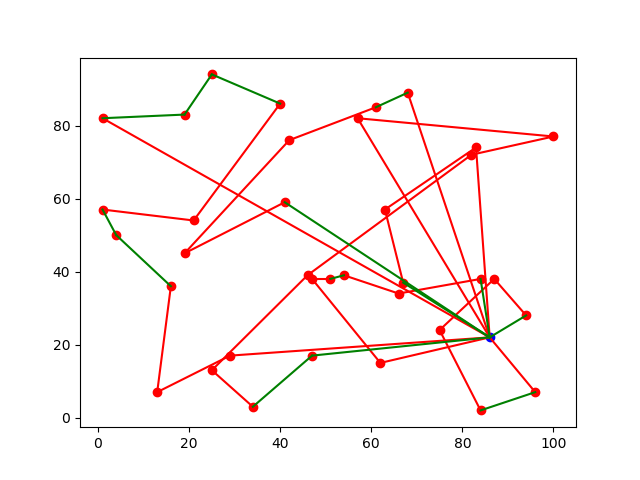
\includegraphics[scale=0.2]{edges010101.png}

	
	\begin{block}{Observations}
	Les bonnes solutions semblent contenir davantage d'arêtes optimales. Le problème est donc de trouver les bons $(\lambda,\mu,\nu)$...
	\end{block}
  \end{column}

 \end{columns}

\end{frame}

\begin{frame}{Protocole}
\begin{alertblock}{Questions}
\begin{itemize}
\item Combien de solutions dans l'échantillon ?
\item Combien de solutions pour apprendre ?
\item Comment choisir les arêtes à conserver ?
\end{itemize}
\end{alertblock}
\end{frame}

\begin{frame}{Protocole}

\begin{block}{Combien de solutions dans l'échantillon ?}
\begin{itemize}
\item Considérer tous les $(\lambda,\mu,\nu)$ (8820 triplets);
\item Tirer $N$ $(\lambda,\mu,\nu)$ aléatoirement. \textcolor{green}{$N \in [50,100,500]$};
\end{itemize}
\end{block}

\begin{block}{Quelles solutions pour apprendre ?}
\begin{itemize}
\item Tout l'échantillon (Tout);
\item $x\%$ des meilleures solutions : quantité privilégiée (Quan$_{x}$);
\item Solutions avec coût inférieur à $c_{min} + (c_{max}-c_{min})\frac{x}{100}$ : qualité privilégiée (Qual$_{x}$);
\end{itemize}
On choisit \textcolor{green}{$x = 10$}
\end{block}
\end{frame}

\begin{frame}{Comment choisir les arêtes à conserver ?}
On initialise une matrice à 0.
Pour chaque arête (i,j), on incrémente la valeur [i][j] de la matrice.

\centering
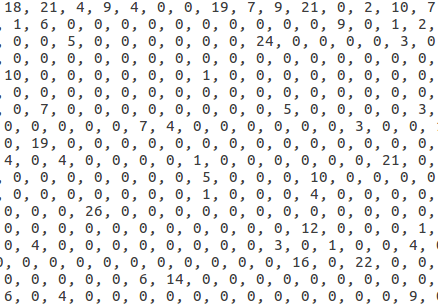
\includegraphics[scale=0.25]{sousmatrice.png}

\begin{columns}[t]

  \begin{column}{4cm}
  	\centering
  	Rang
	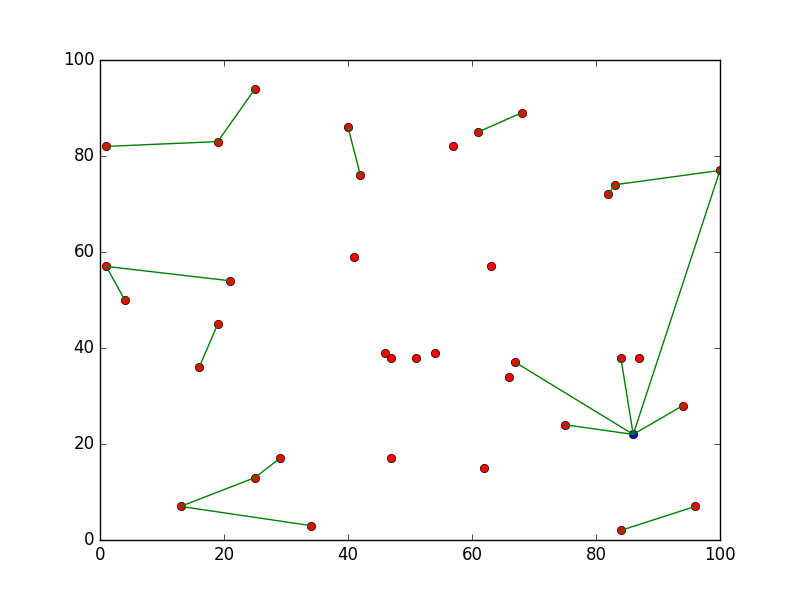
\includegraphics[scale=0.2]{edges_rang.png}
 

  \end{column}
  
 
  \begin{column}{4cm}
  	\centering
  	Seuil
	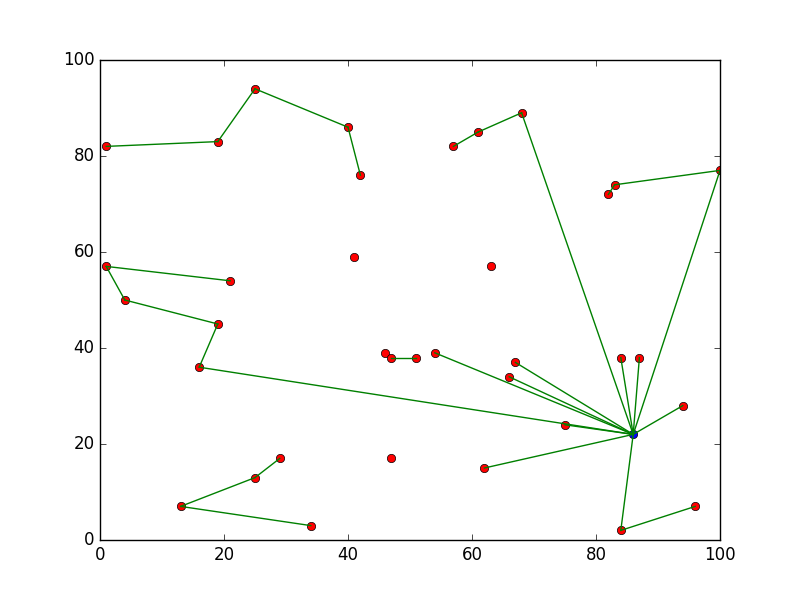
\includegraphics[scale=0.2]{edges_seuil.png}
	
  \end{column}
\end{columns}  
\end{frame}

\begin{frame}{Comment choisir les arêtes à conserver ?}
Deux possibilités pour choisir les arêtes à conserver :
\begin{block}{Critères de choix}
\begin{itemize}
\item Conserver les $rg$ premières arêtes dans la matrice (Rang). \textcolor{green}{$rg \in [10,20,n/2]$};
\item Conserver $(i,j) \Leftrightarrow MAT[i][j] > seuil$ (Seuil). \textcolor{green}{$seuil \in [S_{lb}/2,3S_{lb}/4]$}, $S_{lb}$ (Size learning base) est la taille de la base d'apprentissage.
\end{itemize}
\end{block}
\end{frame}







\subsection{Validation}
\begin{frame}{Résultats A-n37-k06, critère Seuil}

\begin{table}[H]

\begin{tabular}{|@{}c@{}|@{}c@{}|@{}c@{}|@{}c@{}|@{}c@{}||@{}c@{}|@{}c@{}|@{}c@{}|@{}c@{}||@{}c@{}|@{}c@{}|@{}c@{}|@{}c@{}|}

\hline
 & \multicolumn{4}{c|}{Quan$_{10}$} & \multicolumn{4}{c|}{Qual$_{10}$} & \multicolumn{4}{c|}{Tout} \\
 \hline
 & Seuil & Arêtes & Corr & Prop & Seuil & Arêtes & Corr & Prop & Seuil & Arêtes & Corr & Prop \\
 \hline
 50 & 3 & 34 & 21 & 0.5 & 11 & 33 & 21 & 0.50 & 25 & 23 & 15 & 0.35 \\
 \cline{2-13} 
    & 4 & 23 & 14 & 0.33 & 17 & 17 & 12 & 0.28 & 38 & 10 & 7 & 0.16 \\
  \hline
   100 & 5 & 30 & 21 & 0.5 & 15 & 31 & 23 & 0.55 & 50 & 24 & 17 & 0.40 \\
 \cline{2-13} 
    & 8 & 16 & 15 & 0.36 & 23 & 17 & 14 & 0.33 & 75 & 6 & 6 & 0.14 \\
  \hline
   500 & 25 & 32 & 24 & 0.57 & 58 & 31 & 22 & 0.52 & 250 & 22 & 15 & 0.36 \\
 \cline{2-13} 
    & 38 & 15 & 14 & 0.33 & 88 & 20 & 16 & 0.38 & 375 & 7 & 7 & 0.18 \\
  \hline
   Complet & 400 & 33 & 24 & 0.57 & 732 & 30 & 23 & 0.55 & 4000 & 25 & 16 & 0.38 \\
 \cline{2-13} 
    & 600 & 15 & 14 & 0.33 & 1097 & 18 & 16 & 0.38 & 6000 & 9 & 6 & 0.14 \\
  \hline

\end{tabular}
\end{table}
\begin{itemize}
\item Taille de l'échantillon ne semble pas avoir d'influence sur les résultats (\emph{prop} reste semblable quel que soit la taille de l'échantillon).
\item Avec base \emph{Tout} : valeurs de \emph{prop} plus basses $\rightarrow$ pas la peine d'utiliser tout l'échantillon.
\end{itemize}

Remarque : Base Quan$_{10}$ trop petite avec échantillon 50 ou 100.


\end{frame}

\begin{frame}{Résultats A-n37-k06, critère Rang}
\begin{table}[H]

\begin{tabular}{|@{}c@{}|@{}c@{}|@{}c@{}|@{}c@{}||@{}c@{}|@{}c@{}|@{}c@{}||@{}c@{}|@{}c@{}|@{}c@{}|}

\hline
 & \multicolumn{3}{c|}{Quan$_{10}$} & \multicolumn{3}{c|}{Qual$_{10}$} & \multicolumn{3}{c|}{Tout} \\
 \hline
 & Rang & Corr & Prop & Rang & Corr & Prop & Rang & Corr & Prop \\
 \hline
 50 & 10  & 6 & 0.14 & 10  & 6 & 0.14 & 10  & 7 & 0.16  \\
 \cline{2-10} 
    & 20 & 13 & 0.31 & 20  & 13 & 0.32 & 20  & 13 & 0.31  \\
 \cline{2-10} 
    & 18 & 12 & 0.28 & 18 & 13 & 0.3 & 18 & 12 & 0.28  \\
  \hline
   100 & 10  & 9 & 0.21 & 10  & 9 & 0.21 & 10  & 10 & 0.24  \\
 \cline{2-10} 
    & 20 & 16 & 0.38 & 20 & 16 & 0.38 & 20 & 15 & 0.36  \\
  \cline{2-10} 
    & 18 & 13 & 0.3 & 18 & 13 & 0.3 & 18 & 12 & 0.29  \\
  \hline
   500 & 10  & 9 & 0.21 & 10  & 10 & 0.24 & 10  & 9 & 0.21  \\
 \cline{2-10} 
    & 20 & 16 & 0.38 & 20 & 16 & 0.38 & 20 & 15 & 0.36  \\
  \cline{2-10} 
    & 18 & 13 & 0.3 & 18 & 13 & 0.3 & 18 & 12 & 0.28  \\
  \hline
   Complet & 10 & 8 & 0.19 & 10 & 9 & 0.21 & 10 & 7 & 0.17  \\
 \cline{2-10} 
    & 20 & 14 & 0.33 & 20 & 14 & 0.33 & 20 & 14 & 0.33  \\
  \cline{2-10} 
    & 18 & 12 & 0.29 & 18 & 12 & 0.29 & 18 & 12 & 0.29  \\
  \hline

\end{tabular}
\end{table}

Les 3 bases fournissent des valeurs \emph{prop} similaires.


\end{frame}


\begin{frame}{Résultats A-n65-k09, critère Seuil}

\begin{table}[H]

\begin{tabular}{|@{}c@{}|@{}c@{}|@{}c@{}|@{}c@{}|@{}c@{}||@{}c@{}|@{}c@{}|@{}c@{}|@{}c@{}||@{}c@{}|@{}c@{}|@{}c@{}|@{}c@{}|}

\hline
 & \multicolumn{4}{c|}{Quan$_{10}$} & \multicolumn{4}{c|}{Qual$_{10}$} & \multicolumn{4}{c|}{Tout} \\
 \hline
 & Seuil & Arêtes & Corr & Prop & Seuil & Arêtes & Corr & Prop & Seuil & Arêtes & Corr & Prop \\
 \hline
 50 & 3 & 73 & 43 & 0.59 & 10 & 64 & 44 & 0.60 & 25 & 40 & 31 & 0.43 \\
 \cline{2-13} 
    & 4 & 61 & 40 & 0.55 & 15 & 39 & 29 & 0.40 & 38 & 14 & 9 & 0.13 \\
  \hline
   100 & 5 & 70 & 44 & 0.6 & 22 & 58 & 42 & 0.58 & 50 & 43 & 33 & 0.45 \\
 \cline{2-13} 
    & 8 & 63 & 41 & 0.56 & 33 & 36 & 28 & 0.39 & 75 & 15 & 10 & 0.14 \\
  \hline
   500 & 25 & 71 & 43 & 0.59 & 111 & 56 & 41 & 0.56 & 250 & 45 & 35 & 0.48 \\
 \cline{2-13} 
    & 38 & 60 & 40 & 0.55 & 167 & 35 & 28 & 0.39 & 375 & 14 & 9 & 0.13 \\
  \hline
   Complet & 400 & 62 & 41 & 0.56 & 1005 & 56 & 40 & 0.55 & 4000 & 45 & 35 & 0.48 \\
 \cline{2-13} 
    & 600 & 15 & 14 & 0.33 & 1508 & 35 & 28 & 0.39 & 6000 & 13 & 9 & 0.12 \\
  \hline

\end{tabular}


\end{table}

Si trop d'arêtes renvoyées $\rightarrow$ Solutions infaisables ? (futurs tests)


\end{frame}

\begin{frame}{Résultats A-n65-k09, critère Rang}
\begin{table}[H]

\begin{tabular}{|@{}c@{}|@{}c@{}|@{}c@{}|@{}c@{}||@{}c@{}|@{}c@{}|@{}c@{}||@{}c@{}|@{}c@{}|@{}c@{}|}

\hline
 & \multicolumn{3}{c|}{Quan$_{10}$} & \multicolumn{3}{c|}{Qual$_{10}$} & \multicolumn{3}{c|}{Tout} \\
 \hline
 & Rang & Corr & Prop & Rang & Corr & Prop & Rang & Corr & Prop \\
 \hline
 50 & 10  & 6 & 0.08 & 10  & 7 & 0.1 & 10  & 7 & 0.1  \\
 \cline{2-10} 
    & 20 & 14 & 0.2 & 20  & 15 & 0.21 & 20  & 14 & 0.19  \\
 \cline{2-10} 
    & 33 & 23 & 0.32 & 33 & 26 & 0.36 & 33 & 24 & 0.33  \\
  \hline
   100 & 10  & 6 & 0.08 & 10  & 7 & 0.1 & 10  & 7 & 0.1  \\
 \cline{2-10} 
    & 20 & 16 & 0.22 & 20 & 16 & 0.22 & 20 & 14 & 0.19  \\
  \cline{2-10} 
    & 33 & 26 & 0.36 & 33 & 26 & 0.36 & 33 & 25 & 0.34  \\
  \hline
   500 & 10  & 7 & 0.1 & 10  & 7 & 0.1 & 10  & 6 & 0.08  \\
 \cline{2-10} 
    & 20 & 17 & 0.23 & 20 & 15 & 0.21 & 20 & 13 & 0.18  \\
  \cline{2-10} 
    & 33 & 27 & 0.37 & 33 & 26 & 0.36 & 33 & 25 & 0.34  \\
  \hline
   Complet & 10 & 7 & 0.1 & 10 & 7 & 0.1 & 10 & 6 & 0.08  \\
 \cline{2-10} 
    & 20 & 17 & 0.23 & 20 & 17 & 0.23 & 20 & 13 & 0.18  \\
  \cline{2-10} 
    & 33 & 27 & 0.37 & 33 & 27 & 0.37 & 33 & 25 & 0.34  \\
  \hline

\end{tabular}
\end{table}

De nouveau les 3 bases renvoient des résultats similaires. 
\end{frame}

\begin{frame}{Résultats P-n101-k04, critère Seuil}

\begin{table}[H]

\begin{tabular}{|@{}c@{}|@{}c@{}|@{}c@{}|@{}c@{}|@{}c@{}||@{}c@{}|@{}c@{}|@{}c@{}|@{}c@{}||@{}c@{}|@{}c@{}|@{}c@{}|@{}c@{}|}

\hline
 & \multicolumn{4}{c|}{Quan$_{10}$} & \multicolumn{4}{c|}{Qual$_{10}$} & \multicolumn{4}{c|}{Tout} \\
 \hline
 & Seuil & Arêtes & Corr & Prop & Seuil & Arêtes & Corr & Prop & Seuil & Arêtes & Corr & Prop \\
 \hline
 50 & 3 & 93 & 65 & 0.62 & 5 & 83 & 66 & 0.64 & 25 & 71 & 61 & 0.59 \\
 \cline{2-13} 
    & 4 & 54 & 44 & 0.42 & 8 & 42 & 37 & 0.36 & 38 & 24 & 21 & 0.20  \\
  \hline
   100 & 5 & 80 & 66 & 0.64 & 9 & 79 & 66 & 0.63 & 50 & 72 & 62 & 0.60 \\
 \cline{2-13} 
    & 8 & 45 & 41 & 0.40 & 14 & 42 & 39 & 0.38 & 75 & 24 & 22 & 0.21 \\
  \hline
   500 & 25 & 83 & 69 & 0.67 & 44 & 81 & 68 & 0.66 & 250 & 72 & 63 & 0.60 \\
 \cline{2-13} 
    & 38 & 43 & 39 & 0.38 & 67 & 39 & 36 & 0.35 & 375 & 22 & 20 & 0.19 \\
  \hline
   Complet & 400 & 87 & 73 & 0.7 & 411 & 85 & 71 & 0.68 & 4000 & 70 & 60 & 0.58 \\
 \cline{2-13} 
    & 600 & 42 & 39 & 0.38 & 616 & 41 & 38 & 0.37 & 6000 & 23 & 21 & 0.2 \\
  \hline

\end{tabular}


\end{table}

Plus la taille de l'instance augmente, et plus la proportion d'arêtes optimales  renvoyées présentes dans la solution optimale est grande.

\end{frame}

\begin{frame}{Résultats P-n101-k04, critère Rang}
\begin{table}[H]

\begin{tabular}{|@{}c@{}|@{}c@{}|@{}c@{}|@{}c@{}||@{}c@{}|@{}c@{}|@{}c@{}||@{}c@{}|@{}c@{}|@{}c@{}|}

\hline
 & \multicolumn{3}{c|}{Quan$_{10}$} & \multicolumn{3}{c|}{Qual$_{10}$} & \multicolumn{3}{c|}{Tout} \\
 \hline
 & Rang & Corr & Prop & Rang & Corr & Prop & Rang & Corr & Prop \\
 \hline
 50 & 10  & 8 & 0.08 & 10  & 8 & 0.08 & 10  & 8 & 0.08 \\
 \cline{2-10} 
    & 20 & 18 & 0.17 & 20  & 17 & 0.16 & 20 & 18 & 0.17  \\
 \cline{2-10} 
    & 50 & 43 & 0.41 & 50 & 44 & 0.43 & 50 & 44 & 0.43  \\
  \hline
   100 & 10  & 8 & 0.08 & 10  & 8 & 0.08 & 10  & 8 & 0.08  \\
 \cline{2-10} 
    & 20 & 18 & 0.17 & 20 & 18 & 0.17 & 20 & 18 & 0.17  \\
  \cline{2-10} 
    & 50 & 46 & 0.44 & 50 & 46 & 0.44 & 50 & 46 & 0.44  \\
  \hline
   500 & 10  & 8 & 0.08 & 10  & 8 & 0.08 & 10  & 8 & 0.08  \\
 \cline{2-10} 
    & 20 & 18 & 0.17 & 20 & 18 & 0.17 & 20 & 18 & 0.17  \\
  \cline{2-10} 
    & 50 & 46 & 0.44 & 50 & 46 & 0.44 & 50 & 46 & 0.44  \\
  \hline
   Complet & 10  & 8 & 0.08 & 10  & 8 & 0.08 & 10  & 8 & 0.08  \\
 \cline{2-10} 
    & 20 & 18 & 0.17 & 20 & 18 & 0.17 & 20 & 18 & 0.17  \\
  \cline{2-10} 
    & 50 & 46 & 0.44 & 50 & 46 & 0.44 & 50 & 46 & 0.44  \\
  \hline

\end{tabular}
\end{table}
Il faut choisir un rang dépendant de la taille de l'instance (rangs fixés à 10 ou 20 ne revoient plus de bons résultats).
\end{frame}

\section{Intégration des connaissances}

\subsection{Contribution}

\begin{frame}{Où intégrer la connaissance}
Intégration de connaissance lors de la construction de la solution initiale :
\begin{columns}[t]

  \begin{column}{4cm}
  	\centering
	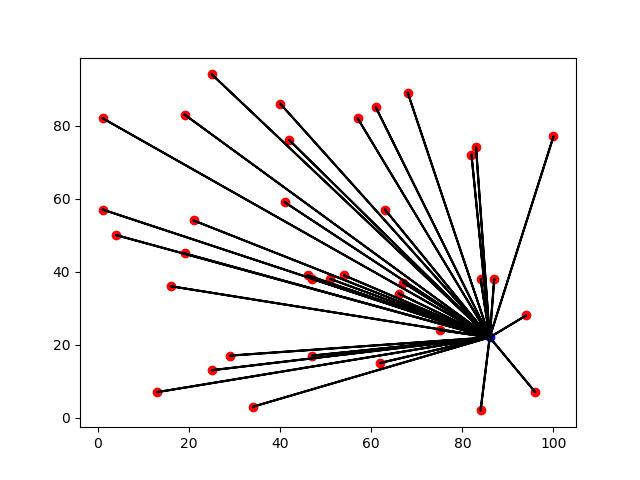
\includegraphics[scale=0.27]{CWinit.png}
 
 	Initialisation habituelle de CW
  \end{column}
  
 
  \begin{column}{4cm}
  	\centering
	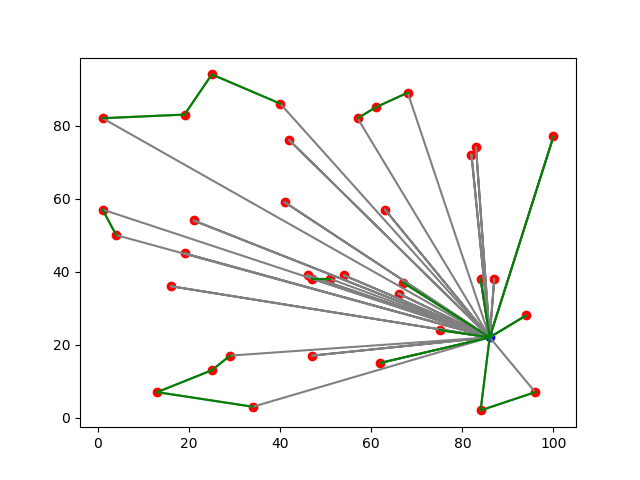
\includegraphics[scale=0.27]{learning.png}
	
	Initialisation de CW après apprentissage ($Init$)
  \end{column}
\end{columns}

On appliquera ensuite CW à $Init$ $\rightarrow$ $(\lambda,\mu,\nu)$ ?

On choisit $(\lambda^*,\mu^*,\nu^*)$ qui a donné le meilleur CW dans l'échantillon (pour l'apprentissage). 
\end{frame}

\begin{frame}{\emph{Learning Heuristic}}
LearnHeuristic (LH)

\begin{algorithm}[H]
\DontPrintSemicolon % Some LaTeX compilers require you to use \dontprintsemicolon instead
$(\lambda^*,\mu^*,\nu^*), Init \gets Apprentissage$\;
$newBase \gets []$\;
\For {$i \gets 1$ \textbf{to} $10$} {
	\If {$i = 1$} {
		$Sol \gets H_c(Init,I,D,\lambda^*,\mu^*,\nu^*)$\;
		$newBase \gets newBase \cup Sol$\;
	}
	\Else {
		Déterminer $Init$ avec les connaissances de $newBase$\;
		 $Sol \gets H_c(Init,I,D,\lambda^*,\mu^*,\nu^*)$\;
		$newBase \gets newBase \cup Sol$\;
	}
}
\Return{La meilleure solution}\;
\end{algorithm}
\end{frame}

\subsection{Validation}
\begin{frame}{Résultats}

\begin{block}{Choix pour apprentissage}
\begin{itemize}
\item Taille échantillon : 100
\item Base : Qual$_{10}$
\item Critère : Rang = $n/2$
\end{itemize}

\end{block}
\begin{table}[H]

\begin{tabular}{|@{}c@{}|@{}c@{}|@{}c@{}|@{}c@{}|@{}c@{}|@{}c@{}|@{}c@{}|@{}c@{}|@{}c@{}|@{}c@{}|}
   \hline
    & \multicolumn{3}{c|}{A-n37-k06} & \multicolumn{3}{c|}{A-n65-k09} & \multicolumn{3}{c|}{P-n101-k04} \\
   \hline
   Connaissances & Best & Mean$_5$ & Time & Best & Mean$_5$ & Time & Best & Mean$_5$ & Time \\
   \hline
   Sans &  963 & 974 & 805 & 1189 & 1236 & 776 & 696 & 708 & 1739  \\   
   \hline
   Avec & 950 & 966 & 1073 (3) & 1186 & 1193 & 911 (8) & 694 & 704 & 1533 (78) \\
   \hline
\end{tabular}
\end{table}
\begin{exampleblock}{Bilan}
L'intégration de connaissance semble apporter de meilleurs résultats
\end{exampleblock}
\end{frame}

\begin{frame}{Limites}
\begin{itemize}
\item Choix de meilleurs valeurs pour l'apprentissage (Taille échantillon, base, critère);
\item Pas beaucoup de solutions pour nouvel apprentissage (avec $newBase$);
\item Toujours même triplet $(\lambda^*,\mu^*,\nu^*)$ utilisé.
\end{itemize}
\end{frame}

\begin{frame}{Prochain algorithme}
\begin{algorithm}[H]
\DontPrintSemicolon % Some LaTeX compilers require you to use \dontprintsemicolon instead
$(\lambda^*,\mu^*,\nu^*), Init \gets Apprentissage()$\;
$newBase \gets []$\;
\For {$i \gets 1$ \textbf{to} $10$} {
	\If {$i = 1$} {
		\textcolor{rouge} {
		\For {$j \gets 1$ \textbf{to} $10$} {
			$Sol \gets H_c(Init,I,D,\lambda^*,\mu^*,\nu^*)$\;
			$newBase \gets newBase \cup Sol$\;
			}	
		}
	}
	\Else {
		Déterminer $Init$ avec les connaissances de $newBase$\;
		\textcolor{rouge}{
		$(\lambda^*,\mu^*,\nu^*), Init \gets Apprentissage(Init)$\;
		}
		\textcolor{rouge}{
		\For {$j \gets 1$ \textbf{to} $10$} {
		 	$Sol \gets H_c(Init,I,D,\lambda^*,\mu^*,\nu^*)$\;
			$newBase \gets newBase \cup Sol$\;
		}
	}
	}
}
\Return{La meilleure solution}\;
\end{algorithm}
\end{frame}

\end{document}